\documentclass{article}
\usepackage{fullpage}
\usepackage{graphicx}
\title{Design Document}
\author{Ryan Wells - 1002253w}
\pagestyle{empty}
\begin{document}
\pagestyle{empty}
\maketitle
\subsection*{System Design}
The design choice of this network driver has been based around the
idea of fairness to all users with the intent of keeping as many
packets in flight at any moment in time. This is achieved by the
following factors.
\subsubsection*{Outgoing Buffer}
An outgoing buffer, herein referred to as ``SendBuffer'', of size
MAX\_PID+1 is a Bounded Buffer which contains the Packet Descriptor
yet to be sent onto
the network. Ideally, with further analysis of the application
domain, a more appropriate number could be picked that is not
dependant on the number of applications but rather on the total number
of free packets available. This would mean that on large systems the size
of the buffer does not vastly overcompensate for the number of
packets available to the Driver and Applications. 
\subsubsection*{Incoming Buffer}
An incoming buffer, herein referred to as ``RecvArray'', is an array
of size MAX\_PID+1 of Bounded Buffers each of size 1 which will
contain one packet for each process as it is received from the
network. Only one packet is kept for each process to encourage
processes to be prompt in retrieving their packets from the network
and to achieve a greater fairness to all programs operating on the
network. Initial attempts to use a Thread Safe Array were less than
fruitful due to compile time uncertainties of size, and creation of
mutex locking for this unknown sized array seemed inefficient. With
more time this approach may have been successful but the decision was
made that the benefits of this result were not worth the time, and so
an array of Bounded Buffers each of size 1 was decided. The RecvArray
is indexed by PID.
\subsubsection*{Sending Thread}
The Sending Thread polls the SendBuffer to see if there is anything to
send to the network device. If there is then the Sending Thread will
remove this from the SendBuffer and attempt to send along the network
device. If a send is unsucessful then an exponential backoff occurs
three times and if still unsucessful gives up, returns the Packet
Descriptor to the Store and continues with the next item in the
SendBuffer. If successful then the Packet Descriptor is also returned
to the Store as per the specification. There is a blocking put to the
Store as every packet should end up back in the store or there may be
a potentially severe implications in the Receiving section if there is
a shortage. Logically, there also cannot exist more Packet Descriptors
in the system than can be held by the Store, so the put should never
actually block and hence the blocking and non blocking methods
are now analogous. Because the guarantee of success is implied I do
not need a return value from the put operation, so blocking was chosen.
\subsubsection*{Receiving Threads}
The Receiving Threads are two threads which run the exact same
function inside the system. The main reason for having two threads
receiving fron the network device is to try to ensure that there will
always be one thread waiting on a packet from the network. This is
achieved by constructing a mutex around the send functionality of the
network device alowing one thread exclusive access to the
functionality while the other blocks waiting for the former thread to
release. The mutex is imediately released after a packet is received
from the network and the waiting thread will obtain this mutex the
next time it is scheduled and begin the setup and waiting for the
network device immediately after this. This design decision was made
to ensure that if there is any delay in other parts of the system
(obtaining a new packet for the next listen on the socket or obtaining
a mutex lock for the correct Bounded Buffer to put the fresh packet
onto) then this will not impact on the overall functionality of the
driver. This is designed with handling a ``burst'' of incoming Packet
Descriptors in mind - packets should not be dropped due to system
incompetency. 

A Receiving Thread has space for two Packet Descriptors at any
one time, however it only holds two for a very small portion of its
cycle. Upon receiving a Packet from the network, it releases the mutex
and then immediately attempts to get a second Packet Descriptor from
the Store using a non blocking get. If this retrieval of a new Packet
Descriptor was
successful, then the Receiving Thread will attempt to put the first
Packet Descriptor into the RecvArray - it will only insert it if the
array element (Bounded Buffer) relating to the Packet Descriptors PID
is empty. This encourages the processes to collect their Packet
Descriptors promptly and also keeps the Packet Descriptors flowing
through the system. The new packet then becomes the next to be used on
the network device. If the retrieval of a new Packet Descriptor was
unsuccessful then the Packet Descriptor is ``dropped'' by being
immediately reused to listen on the socket. This ensures that the
issue of a shortage of packets is not propogated down into the network
device and the network device is still being kept busy - at all times
the network device must view the network driver as working
correctly. Eventually, Packet Descriptors will become free and will
allow the Receive Threads to properly execute.

\subsubsection*{Non Blocking Send and Receive}
The blocking send works returns true only if there is room in the
SendBuffer to hold the Packet Descriptor. The Packet Descriptor is
added if this is the case, and not if there is not room. No blocking
other than obtaining the mutex for the SendBuffer happens.
The blocking receive returns the Packet Descriptor in the Bounded
Buffer, at index PID of the requesting process in the RecvArray, if
one exists and returns null if not. No blocking other than obtaining
the mutex for the Bounded Buffer for this PID happens.

\subsubsection*{Blocking Send and Receive}
The blocking send blocks until there is room in the SendBuffer to put
its Packet Descriptor and then returns.

The blocking receive blocks until there is a Packet Descriptor waiting
in the Bounded Buffer at array index PID (of the requesting process) of
the RecvArray and then returns the Packet Descriptor.

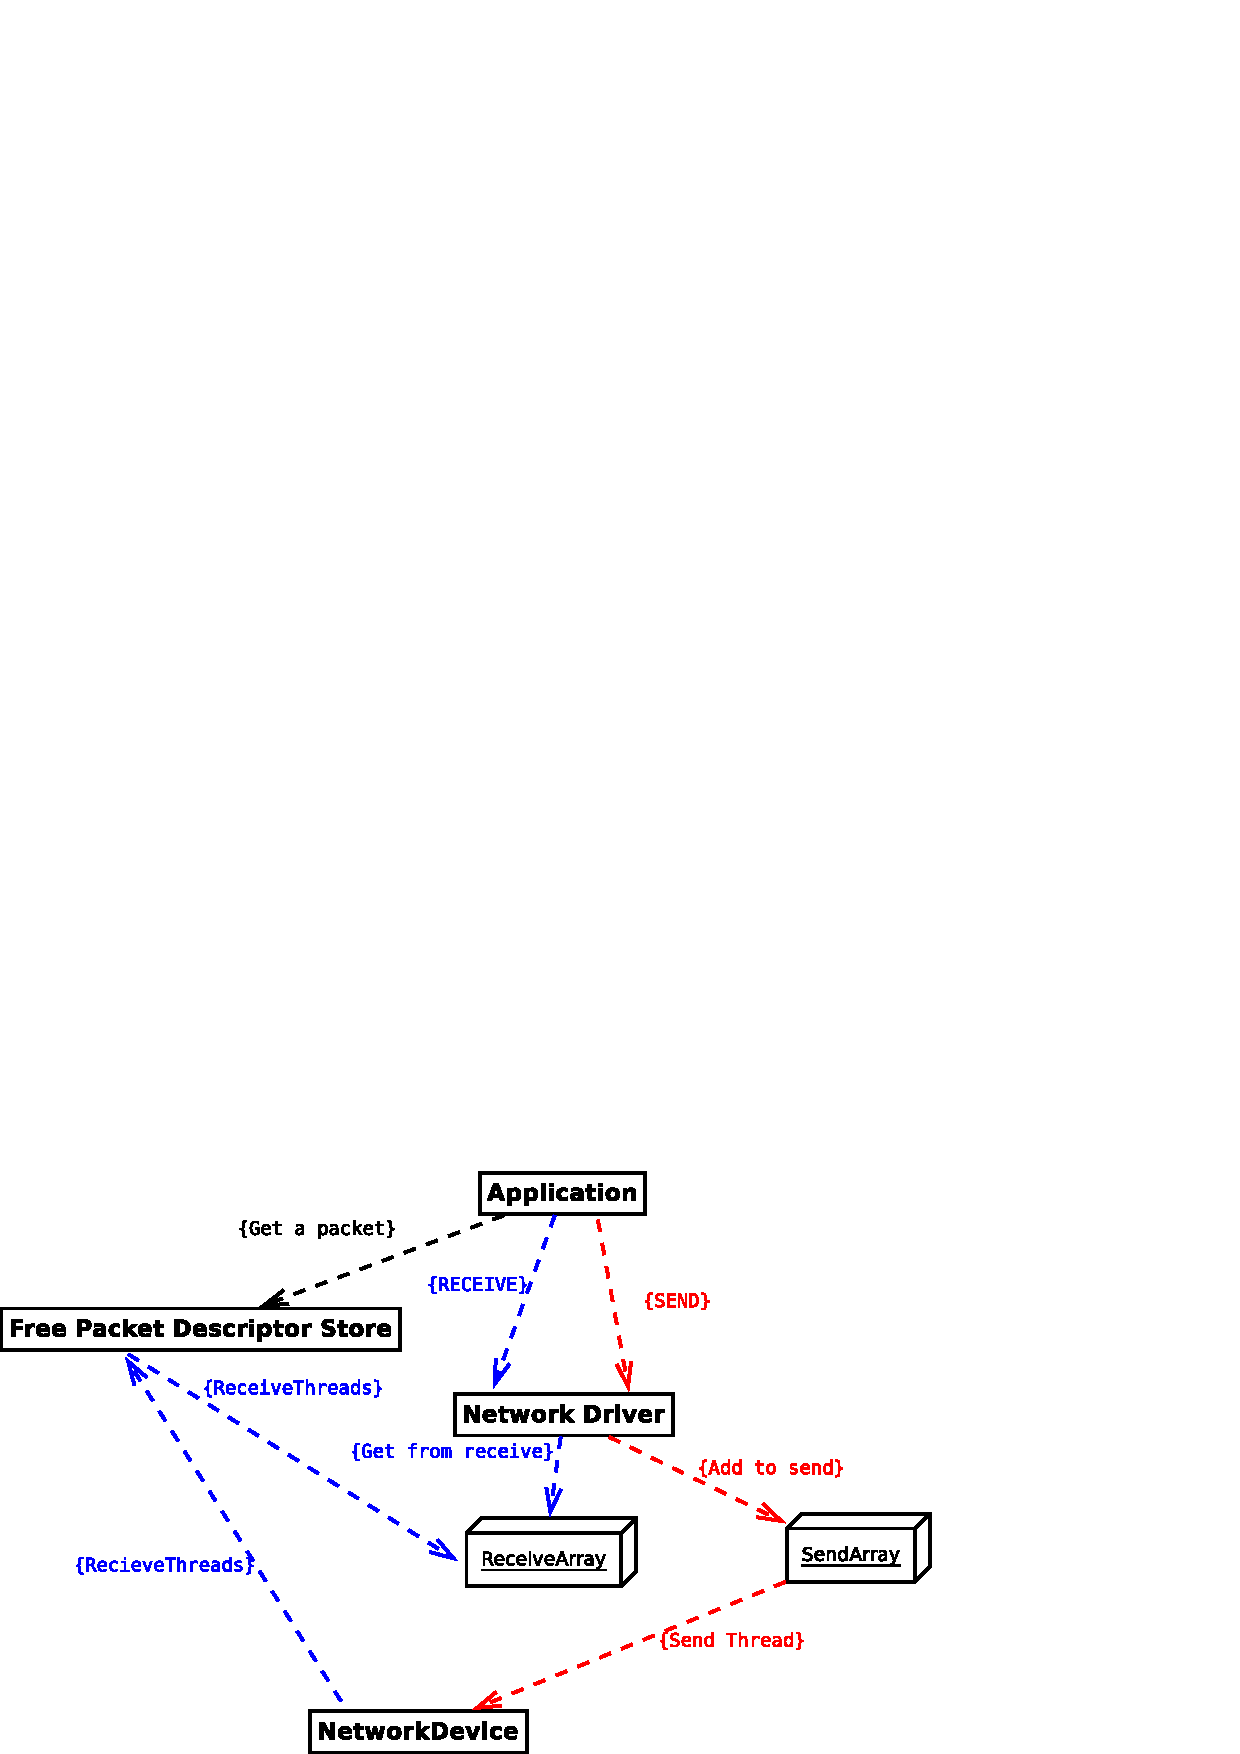
\includegraphics[clip=true,trim=100 50 200 25, width=0.45\textwidth,angle=270]{Diagram.pdf}
\end{document}
